\chapter{Appendix}
\section{Gamma functions}
a gamma distribution can be described by the equation: 
\begin{equation}
	f(x;\alpha,\beta)  = \frac{\beta^\alpha x^{\alpha-1} e^{-\beta x}}{\Gamma (\alpha)}
\end{equation}
where $\alpha$ is known as the shape parameter, and $\beta$ is known as the inverse scale parameter($\beta = 1/\theta$ where $\theta$ is the scale parameter)). $\Gamma(x)$ is described by;
\begin{align}
	\Gamma(n) &= (n-1)! \hspace{1cm} n\in \mathds{Z} \\
	&= \int_{0}^{\infty}x^{n-1} e^{-x} dx\hspace{1cm}   n\in \mathds{C}
\end{align}
taking the derivative of the gamma distribution we get:
\begin{align}
	f' & = \frac{d}{dx}\left(\beta^\alpha e^{-\beta x}x^{\alpha-1} \right) \\
	& =\beta^\alpha \left( x^{\alpha -1} \left(\frac{d}{dx}\left( e^{-\beta x} \right) \right) + e^{-\beta x }\left( \frac{d}{dx}\left( x^{\alpha -1} \right) \right) \right)\\
	& = \beta^\alpha \left( 	(\alpha -1 ) e^{-\beta x} x^{\alpha -2} + -\beta x^{\alpha -1}e^{-\beta x}    	\right) \\
	%& = 
\end{align}
equating to zero to find a maximum we get;
\begin{align}
	0 &= \beta^\alpha \left( 	(\alpha -1 ) e^{-\beta x} x^{\alpha -2} + -\beta x^{\alpha -1}e^{-\beta x}   \right) \\
	&=  (\alpha -1 ) e^{-\beta x} x^{\alpha -2} + -\beta x^{\alpha -1}e^{-\beta x} \\
	&=  (\alpha -1 ) x^{\alpha -2} + -\beta x^{\alpha -1} \\
	&= \frac{(\alpha -1 )x^{\alpha-1}}{x} - \beta x^{\alpha -1} \\
	&= \frac{\alpha  -1}{x} - \beta \\
	x & = \frac{\alpha -1}{\beta}
\end{align}


So a critical point (the maximum) occurs at $(\alpha -1)/\beta$ which corresponds to a maximum of;
\begin{align}
f\left( \frac{\alpha-1}{\beta};\alpha,\beta \right) & = \frac{\beta^\alpha \left( \frac{\alpha-1}{\beta}\right)^{\alpha -1} e^{-\beta \frac{\alpha-1}{\beta}}}{\Gamma(\alpha)}\\
\end{align}

For the project, gamma functions were fit to the distributions displacements by different metrics, for walks of a certain length using scipy.stats.gamma. Using this package, the form of the maximum after fit, is;

Where $loc$ is the offset of the centre of the distribution.
Scipy.stats.gamma also gives us the fit parameters in the form $[\alpha, loc, \theta ]$ or $[shape, location, scale]$ so theta must also me converted;
\begin{figure}

\end{figure}


		\section{Maths}
		\subsection{Definitions}
		\label{app:pauli}
		Pauli Matrices
		\[
		X = 
		\begin{bmatrix}
		0 & 1 \\
		1 & 0
		\end{bmatrix}
		, Y = 
		\begin{bmatrix}
		0  & -i \\
		i & 0
		\end{bmatrix}
		, Z = 
		\begin{bmatrix}
		1  & 0 \\
		0 & -1
		\end{bmatrix}
		, I = 
		\begin{bmatrix}
		1  & 0 \\
		0 & 1
		\end{bmatrix}
		\label{fig:pauli}
		\]
\subsection{Hadamard Gate}
\label{app:hadamard}
		The Hadamard gate can be used to convert a $\ket{0}$ into $ \frac{1}{\sqrt{2}}(\ket{0} +\ket{1})$ and $\ket{1}$ into $ \frac{1}{\sqrt{2}}(\ket{0} -\ket{1})$.
		It is represented by the transformation matrix:
		\[ H = 
				\frac{1}{\sqrt{2}}\begin{bmatrix}
				1  & 1 \\
				1 & -1
				\end{bmatrix}
				\]
		This transformation allows for concatenated error correcting codes to deal with X and Z errors using the same procedure. 
		\subsection{Homology Classes}
		\label{app:cycles}

		A cycle is a loop. On a torus a homologically nontrivial cycle corresponds to a horizontal or vertical chain extending over the periodic boundary conditions which forms a noncontractibel loop. Any chain homologically equivalent to these chains is also homologically nontrivial. These cycles do not form the boundary of any surface. A trivial cycle is equivalent to any cycle which forms the boundary of a surface. 
		
		A single non-contractible loop cannot be formed from stabilizers; only pairs of loops which form the boundary of a region one dimension higher than the boundary chain itself. Thus, only trivial homologies can be formed from stabilizer measurements. 
		\begin{figure}
		\centering
		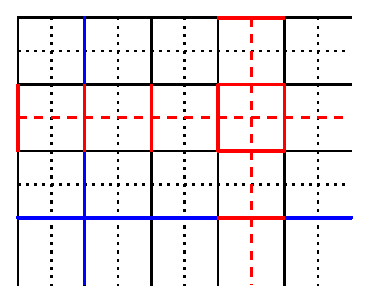
\includegraphics[width = 0.4\textwidth]{figs/errors.eps}
		\caption{This figure shows the 4 nontrivial cycles on the torus. There are conjugate directions for each chain of X and Z operators. Two of the cycles exist on the grid, and 2 exist on the co-grid.}
		\label{fig:errors}
		\end{figure}
		A linear combination of 2 rings around the torus forms the boundary of a 2D surface (an empty cylinder) which is 1D higher than the cycles forming the boundary; which means the homology is trivial.
		
		On the toric code, a homologically nontrivial loop does not commute with the hamiltonian. Trivial loops, such as those created by strings of stabilizers, commmute with the hamiltonian. 
		
\section{Code}
	This section contains small logically important snippets of the code are included here. 800 lines of core code was developed, along with supporting code for data processing, interfacing with code borrowed from Nickerson \cite{Nickerson2014}, and graphical displays.	
	\\\\
	Full code can be found at \url{https://github.com/gorff/Toric-Code-Correlated-Error-Decoder}.
		
		\begin{lstlisting}[language=Python, caption=Applying Uncorrelated Errors, label = code:applyerrors]
def ApplyUncorrelatedErrors( ErrorNum,array,type,L,CorrLen):
	#run across every element in the array
	for i in range(len(array[:,0,0])):
	   for j in range(2):
	       for k in range(len(array[0,0,:])):
	           if random.random() >1-ErrorRate: #rand chance of bitflip
	               array[i,j,k] = -1*array[i,j,k] #apply bitflip if true
	return(array)
		\end{lstlisting}

